
\section{Background theory}

\subsection{Mathematical model (Quasi-steady )}

 One of the widely used mathematical model to predict the system response under galloping is the Quasi-steady state (QSS) model, incorporated by \cite{Parkinson1964} for a square cross section. The equation of motion of the body under galloping is given by Eq. \eqref{equationofmotion}. The forcing term $F_y$ is given by Eq.\eqref{lift equation}.
 
 \begin{figure}
\setlength{\unitlength}{\textwidth}

  \begin{picture}(1,0.23)(0,0.74)
    
  \put(0.2,0.76){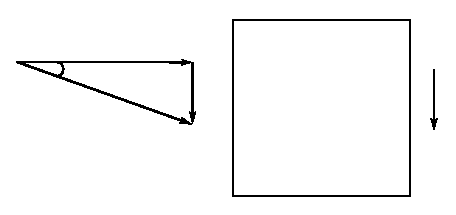
\includegraphics[width=0.5\unitlength]{../FnP/gnuplot/setup-1.eps}}         
      
      
   
 	\put(0.315,0.93){$U$}
 	\put(0.3,0.84){$U_i$}
    \put(0.42,0.88){$\dot{y}$}
    \put(0.28,0.895){ $\theta$}
    \put(0.7,0.87){\small $(+)$}
      	

 	
 	 

     

  \end{picture}

 \caption{Induced angle of attack on the square prism due to the resultant of free-stream velocity of the fluid and transverse velocity of the body.}
    \label{fig:setup_1}
\end{figure}

\begin{equation}
\label{equationofmotion}
(m+m_a)\ddot{y}+c\dot{y}+ky=F_y
\end{equation}

\begin{equation}
\label{lift equation}
F_y=\frac{1}{2}\rho U^2\mathcal{A}C_y
\end{equation}

 In the QSS  model $C_y$ is determined by an interpolating polynomial based on the stationary lift and drag data. The order of the interpolation polynomial has varied from study to study. For  example a $7^{th}$ order was used in \cite{Parkinson1964} and $3^{rd}$ order polynomial was used in \cite{Barrero-Gil2009}. \cite{Ng2005} concluded that using a $7^{th}$ order polynomial is sufficient and a polynomial higher than that of $7^{th}$ order polynomial neither results in a result significantly better result nor does it exhibit an additional amplitudes of oscillation. Thus a $7 ^{th}$ order interpolating polynomial was incorporated in this present study. 

\begin{equation}
\label{cy ploynomial}
C_y(\theta)=a_1\left(\frac{\dot{y}}{U}\right)+a_3\left(\frac{\dot{y}}{U}\right)^3+a_5\left(\frac{\dot{y}}{U}\right)^5+a_7\left(\frac{\dot{y}}{U}\right)^7
\end{equation}

%\begin{equation}
%\label{modified_equation_of_motion}
%\ddot{y}+c^*\dot{y}+k^*y=\frac{1}{2}\rho U^2A
%\end{equation}

\cite{Joly2012} reported a reduction of displacement amplitude at low mass ratios. Therefore in order to account for it a sinusoidal forcing function to the RHS of the oscillator model (Eq. \eqref{equationofmotion})was introduced, in order to represent forcing due to VIV. This method provided satisfactory results with the numerical simulations obtained at low mass ratios. This study, the forcing due to VIV is incorporated using a sinusoidal forcing function $F_0\sin{\omega_{s}t}$ added to the RHS of the equation. $\omega_{s}$ and $F_0$ represents shedding frequency and the maximum force due to shedding respectively. Thus, the final equation is given by Eq. \eqref{final_equation_motion}.    

\begin{equation}
\label{final_equation_motion}
(m{+}m_a)\ddot{y}{+}c{+}\dot{y}{+}ky{=}\frac{1}{2}\rho U^2 \mathcal  {A} \Bigg(a_1\left(\frac{\dot{y}}{U}\right){+}a_3\left(\frac{\dot{y}}{U}\right)^3{+}a_5\left(\frac{\dot{y}}{U}\right)^5{+}a_7\left(\frac{\dot{y}}{U}\right)^7 \Bigg){+} F_0\sin{(\omega_s t)}
\end{equation}

This equation could be solved by time integration methods. In  this study  ``Ode 45" routine in MATLAB was used to obtain the solutions.

\subsection{Calculation of average power}

 The dissipated power due to the mechanical damping could be expressed as the harvested power output assuming that the other  power dissipation due to internal damping such as friction of the system is negligible. Therefore the mean power output could be given by Eq. \eqref{power}. 
  
 
 \begin{equation}
 \label{power}
P_{mean}=\frac{1}{T}\int_{0}^{T}(c\dot{y})\dot{y} dt
 \end{equation}
 
 \begin{figure}

  \setlength{\unitlength}{\textwidth}
  \begin{picture}(1,0.25)(0,0.8)
  
    % % %90
      \put(0.025,0.81){\includegraphics[width=0.5\unitlength]{../FnP/gnuplot/lift_curve_165.eps}}
      \put(0.495,0.81){\includegraphics[width=0.5\unitlength]{../FnP/gnuplot/lift_curve_park.eps}}
 	\put(0.02,0.93){ \large $C_y$} 	
% 	\put(0.56,1.02){ $\theta$}
 	
        \put(0.25,0.8){ $\theta$} 	
        \put(0.75,0.8){ $\theta$}
        
        \put(0.105,1.01){(a)}
        \put(0.565,1.01){(b)}
      \end{picture}

  \caption{Lift coefficient, $C_y$ \JL{$C_y$ is upper case here, lower case on the figure. Make them match what is in the nomenclature}, as a function of incidence angle $\theta$, for a static square cross section. (a) Data from simulations at $Re=165$  (b) data from \cite{Parkinson1964} at $Re=22300$. Points ($\bullet$) are measurements from the simulations. The solid lines in both plots are 7th-order interpolating polynomial used to predict the fluid forcing for the QSS model.}
    \label{fig:lift_curves}
\end{figure}
 \vspace{20mm}
 \begin{table}[ht]

\begin{center}
\setlength{\unitlength}{\textwidth}

\begin{tabular}{c c c c c} % centered columns (4 columns)
\hline\hline %inserts double horizontal lines
\\[0.2ex]
Case & $a_1$ & $a_3$ & $a_5$ & $a_7$ \\ [0.8ex] % inserts table 
%heading
\hline 
\\[0.8ex]% inserts single horizontal line
Re=165 & 1.3 & 125.3 & 1825.73 & 8765.3 \\[0.8ex] % inserting body of the table
Re=22300 & 2.69 & 168 & 1670 & 59900 \\ [1ex] % [1ex] adds vertical space
\hline %inserts single line
\end{tabular}

\caption{Coefficient values used in the 7th order interpolation polynomial for high ($Re=165$) and low ($Re=22300$) Reynolds numbers. These data are used as input data to calculate the RHS of Eq.\ref{final_equation_motion} throughout this study.}
 
\label{table:nonlin} % is used to refer this table in the text
\end{center}
\end{table}


 
\subsection{Parameters used} 
 
The stationary data and the fluid-structure interaction (FSI) data were obtained using a higher order spectral element code which simulate 2D laminar flow. The Reynolds number was kept at 165 as it was pointed out by \cite{Sheard2009} and \cite{Tong2008} that the 3 dimensional transition for a square cylinder occurs at approximately Re=160. $F_0$ was kept at $0.4937$ which was obtained by using a simple linear interpolation on the data presented in \cite{Joly2012}. $\omega_s$ was set to $0.98$ winch was obtained by performing a power spectral analysis of the stationary data at $0^0$. Stationary $C_y$ data were obtained at different angles of attack ranging from $0^0$ to $16^0$. The average power was obtained by using Eq. \eqref{power} with data sets consisting substantial amount of peaks. Power data  at Re=22300 were obtained using input $C_y$ data in \cite{Parkinson1964} in order to provide a comparison between high and low Reynolds numbers. $m^*$ was kept at 1163 for \reynoldsnumber=22300 (Similar as \cite{Parkinson1964}) amd $m^*=20$ for \reynoldsnumber=165. These parameters  were used throughout this study unless otherwise specified. 


 FSI data were obtained for the oscillating (free-vibration) scenario. The Naiver-Stokes equations were solved using an accelerated frame of reference using the previously mentioned code. A three-step time splitting scheme together with high-order Lagrangian polynomials were used to obtain the solution. The details of the method could be found in \cite{Thompson2006,Thompson1996a}. This code was incorporated in \cite{Leontini2011,Leontini2007a}  where it was employed in a fluid-structure interaction problems. 
 
 The computational domain consists of 690 quadrilateral macro elements where majority of the elements were concentrated near the square section. A freestream condition was given to the inlet, top and bottom boundaries and the normal velocity gradient was set to zero at the outlet. A convergence study was performed by changing the order of the polynomial ($p$-refinement) at $U^*=40$ and Re $165$. A 9th order polynomial together with a time step of $\frac{\Delta tU}{D}=0.001$ was sufficient to ensure an accuracy of $2\%$ with regards to amplitude of oscillation.  
 

 
 
 

 
 
 
 









